% Options for packages loaded elsewhere
\PassOptionsToPackage{unicode}{hyperref}
\PassOptionsToPackage{hyphens}{url}
\PassOptionsToPackage{dvipsnames,svgnames,x11names}{xcolor}
%
\documentclass[
]{article}

\usepackage{amsmath,amssymb}
\usepackage{iftex}
\ifPDFTeX
  \usepackage[T1]{fontenc}
  \usepackage[utf8]{inputenc}
  \usepackage{textcomp} % provide euro and other symbols
\else % if luatex or xetex
  \usepackage{unicode-math}
  \defaultfontfeatures{Scale=MatchLowercase}
  \defaultfontfeatures[\rmfamily]{Ligatures=TeX,Scale=1}
\fi
\usepackage{lmodern}
\ifPDFTeX\else  
    % xetex/luatex font selection
  \setmainfont[]{Latin Modern Roman}
  \setmathfont[]{Latin Modern Math}
\fi
% Use upquote if available, for straight quotes in verbatim environments
\IfFileExists{upquote.sty}{\usepackage{upquote}}{}
\IfFileExists{microtype.sty}{% use microtype if available
  \usepackage[]{microtype}
  \UseMicrotypeSet[protrusion]{basicmath} % disable protrusion for tt fonts
}{}
\makeatletter
\@ifundefined{KOMAClassName}{% if non-KOMA class
  \IfFileExists{parskip.sty}{%
    \usepackage{parskip}
  }{% else
    \setlength{\parindent}{0pt}
    \setlength{\parskip}{6pt plus 2pt minus 1pt}}
}{% if KOMA class
  \KOMAoptions{parskip=half}}
\makeatother
\usepackage{xcolor}
\setlength{\emergencystretch}{3em} % prevent overfull lines
\setcounter{secnumdepth}{5}
% Make \paragraph and \subparagraph free-standing
\ifx\paragraph\undefined\else
  \let\oldparagraph\paragraph
  \renewcommand{\paragraph}[1]{\oldparagraph{#1}\mbox{}}
\fi
\ifx\subparagraph\undefined\else
  \let\oldsubparagraph\subparagraph
  \renewcommand{\subparagraph}[1]{\oldsubparagraph{#1}\mbox{}}
\fi


\providecommand{\tightlist}{%
  \setlength{\itemsep}{0pt}\setlength{\parskip}{0pt}}\usepackage{longtable,booktabs,array}
\usepackage{calc} % for calculating minipage widths
% Correct order of tables after \paragraph or \subparagraph
\usepackage{etoolbox}
\makeatletter
\patchcmd\longtable{\par}{\if@noskipsec\mbox{}\fi\par}{}{}
\makeatother
% Allow footnotes in longtable head/foot
\IfFileExists{footnotehyper.sty}{\usepackage{footnotehyper}}{\usepackage{footnote}}
\makesavenoteenv{longtable}
\usepackage{graphicx}
\makeatletter
\def\maxwidth{\ifdim\Gin@nat@width>\linewidth\linewidth\else\Gin@nat@width\fi}
\def\maxheight{\ifdim\Gin@nat@height>\textheight\textheight\else\Gin@nat@height\fi}
\makeatother
% Scale images if necessary, so that they will not overflow the page
% margins by default, and it is still possible to overwrite the defaults
% using explicit options in \includegraphics[width, height, ...]{}
\setkeys{Gin}{width=\maxwidth,height=\maxheight,keepaspectratio}
% Set default figure placement to htbp
\makeatletter
\def\fps@figure{htbp}
\makeatother
% definitions for citeproc citations
\NewDocumentCommand\citeproctext{}{}
\NewDocumentCommand\citeproc{mm}{%
  \begingroup\def\citeproctext{#2}\cite{#1}\endgroup}
\makeatletter
 % allow citations to break across lines
 \let\@cite@ofmt\@firstofone
 % avoid brackets around text for \cite:
 \def\@biblabel#1{}
 \def\@cite#1#2{{#1\if@tempswa , #2\fi}}
\makeatother
\newlength{\cslhangindent}
\setlength{\cslhangindent}{1.5em}
\newlength{\csllabelwidth}
\setlength{\csllabelwidth}{3em}
\newenvironment{CSLReferences}[2] % #1 hanging-indent, #2 entry-spacing
 {\begin{list}{}{%
  \setlength{\itemindent}{0pt}
  \setlength{\leftmargin}{0pt}
  \setlength{\parsep}{0pt}
  % turn on hanging indent if param 1 is 1
  \ifodd #1
   \setlength{\leftmargin}{\cslhangindent}
   \setlength{\itemindent}{-1\cslhangindent}
  \fi
  % set entry spacing
  \setlength{\itemsep}{#2\baselineskip}}}
 {\end{list}}
\usepackage{calc}
\newcommand{\CSLBlock}[1]{\hfill\break\parbox[t]{\linewidth}{\strut\ignorespaces#1\strut}}
\newcommand{\CSLLeftMargin}[1]{\parbox[t]{\csllabelwidth}{\strut#1\strut}}
\newcommand{\CSLRightInline}[1]{\parbox[t]{\linewidth - \csllabelwidth}{\strut#1\strut}}
\newcommand{\CSLIndent}[1]{\hspace{\cslhangindent}#1}

\usepackage{booktabs}
\usepackage{longtable}
\usepackage{array}
\usepackage{multirow}
\usepackage{wrapfig}
\usepackage{float}
\usepackage{colortbl}
\usepackage{pdflscape}
\usepackage{tabu}
\usepackage{threeparttable}
\usepackage{threeparttablex}
\usepackage[normalem]{ulem}
\usepackage{makecell}
\usepackage{xcolor}
\usepackage{arxiv}
\usepackage{orcidlink}
\usepackage{amsmath}
\usepackage[T1]{fontenc}
\makeatletter
\@ifpackageloaded{caption}{}{\usepackage{caption}}
\AtBeginDocument{%
\ifdefined\contentsname
  \renewcommand*\contentsname{Table of contents}
\else
  \newcommand\contentsname{Table of contents}
\fi
\ifdefined\listfigurename
  \renewcommand*\listfigurename{List of Figures}
\else
  \newcommand\listfigurename{List of Figures}
\fi
\ifdefined\listtablename
  \renewcommand*\listtablename{List of Tables}
\else
  \newcommand\listtablename{List of Tables}
\fi
\ifdefined\figurename
  \renewcommand*\figurename{Figure}
\else
  \newcommand\figurename{Figure}
\fi
\ifdefined\tablename
  \renewcommand*\tablename{Table}
\else
  \newcommand\tablename{Table}
\fi
}
\@ifpackageloaded{float}{}{\usepackage{float}}
\floatstyle{ruled}
\@ifundefined{c@chapter}{\newfloat{codelisting}{h}{lop}}{\newfloat{codelisting}{h}{lop}[chapter]}
\floatname{codelisting}{Listing}
\newcommand*\listoflistings{\listof{codelisting}{List of Listings}}
\makeatother
\makeatletter
\makeatother
\makeatletter
\@ifpackageloaded{caption}{}{\usepackage{caption}}
\@ifpackageloaded{subcaption}{}{\usepackage{subcaption}}
\makeatother
\ifLuaTeX
  \usepackage{selnolig}  % disable illegal ligatures
\fi
\usepackage{bookmark}

\IfFileExists{xurl.sty}{\usepackage{xurl}}{} % add URL line breaks if available
\urlstyle{same} % disable monospaced font for URLs
\hypersetup{
  pdftitle={Spatial Modeling of Cardiovascular Disease Incidence Positively Associated with PM2.5},
  pdfauthor={Johan Booc; Christina Kim; Shombit Roy},
  pdfkeywords={Fine Particulate Matter (PM2.5), Cardiovascular Disease
(CVD), Cardiovascular Mortality (CVM)},
  colorlinks=true,
  linkcolor={blue},
  filecolor={Maroon},
  citecolor={Blue},
  urlcolor={Blue},
  pdfcreator={LaTeX via pandoc}}

\usepackage{lineno}
\linenumbers
\usepackage{setspace}
\doublespacing
\newcommand{\runninghead}{A Preprint }
\renewcommand{\runninghead}{CVD Related to PM2.5 }
\title{Spatial Modeling of Cardiovascular Disease Incidence Positively
Associated with PM2.5}
\def\asep{\\\\\\ } % default: all authors on same column
\author{\textbf{Johan Booc}\\Department of Statistics\\Texas A\&M
University\\\\\href{mailto:jbooc24@tamu.edu}{jbooc24@tamu.edu}\asep\textbf{Christina
Kim}\\Department of Statistics\\Texas A\&M
University\\\\\href{mailto:christinaykim3@tamu.edu}{christinaykim3@tamu.edu}\asep\textbf{Shombit
Roy}\\Department of Statistics\\Texas A\&M
University\\\\\href{mailto:shombit123@tamu.edu}{shombit123@tamu.edu}}
\date{}
\begin{document}
\maketitle
\begin{abstract}
Cardiovascular disease (CVD) is the leading cause of death in the United
States. By using a spatial modeling technique (geographically weighted
regression) we observed that the concentration of PM 2.5 is centered in
the Stroke Belt region after adjusting for median household income and
unemployment rates (finding similar correlations studied in the past).
Policymakers and health practitioners can use these results to identify
targeted interventions to curb the increasing rates of CVD, and help to
halt one of the world's deadliest diseases.
\end{abstract}
{\bfseries \emph Keywords}
\def\sep{\textbullet\ }
Fine Particulate Matter (PM2.5) \sep Cardiovascular Disease (CVD) \sep 
Cardiovascular Mortality (CVM)


\section{Introduction}\label{sec-intro}

As cardiovascular disease is the leading cause of death in the US,
numerous past studies have been done on this disease, specifically on
the older population the 65+ year age group. Our study aims to further
investigate the impact, focusing on the 18-44-year-old age population,
since generally, there has been less interest in the effects of CVD on
them.~

Our approach involves analyzing this relationship to produce risk
prediction estimates for our specified age group. There are several
factors involved in influencing the incidence rates of CVD from
genetics, lifestyle, diet, and smoking/alcohol habits. We look into the
covariates - PM 2.5 concentration, median household income, and
unemployment rates - to analyze the spatial variation for our specified
age population, thus decreasing future CVD incidence rates.
Specifically, we focus on PM 2.5 concentration as the world continues to
depend on fossil fuels/natural gas and climate change is an ongoing
concern. Earlier studies such as (Warsito et al. 2018) and (Liu et al.
2020)highlight the modern-day threats from air pollution using a Robust
GWR model and Bayesian-temporal model, respectively. From studying our
covariates, we can examine the effects of certain CVD risk factors for
the year 2015.~

The geographically weighted regression model uses local variables and
weights to produce statistical visualizations of the US's regional
variation between our response variable (CVD deaths) and its covariates.
Other methods, such as the traditional linear regression model and
clustering, have been used in past CVD studies. However, we found the
GWR model allows us to see each covariate's local significance and
magnitude. The spatial distribution aspect of the GWR model highlights
regions that are concentrated with CVD rates, whether incidence
percentage rates are increasing or decreasing, and any significant
correlations. This makes the GWR model efficient in analyzing the
dynamic relationship of CVD rates and the factors that contribute to
it.~

Using a geographically weighted regression approach, the overall outcome
of our study aids policymakers and health practitioners in implementing
the necessary interventions for targeted regions that are being
influenced the most by our covariates. For public health experts, it's
ideal to tailor aid to each specific region of the US first to
eventually reach a national decrease in CVD incidence rates.

\section{Related Works}\label{related-works}

There's a growing popularity of using spatial models in the
epidemiological domain to analyze the distribution and factors of a
disease. The techniques often used differ between studies but all have
the same goal: to reduce the disease incidence and mortality rates.
Statistical regression models are popular methods for CVD studies. The
underlying causes for CVD are dynamic and can be seen as an
interconnected web. (Zelko et al. 2023) examines the relationship
between CVD and covariates similar to our study (air pollution, social
determinants, and county-level data). From using a GWR model, their
results found that counties in the South had the highest exposure to PM
2.5 concentrations whereas counties in the Northeast had the lowest. A
strong correlation was also found between household income, race, and
healthcare access. Overall, there are several causes to consider with
CVD, and where the covariates are concentrated is another important
consideration.

Compared to traditional regression models, the geographically weighted
model (GWR) explores spatial data by considering varied coefficients for
a certain spatial unit (Gebreab and Diez Roux 2012). The GWR model
contains the parameter, neighborhood (also known as bandwidth) and
builds on the weighted least squares method to estimate the regression
coefficients. We want to see values closer to the point of interest
since they carry more weight, thus having a greater influence.~

The Ordinary Least Squares (OLS) model is a popular choice of method for
public health studies because it generates the regression coefficients
on a global scale and captures the average differences between
covariates. However, this means spatial variability between units can be
easily hidden for the OLS model. Our paper acknowledges that PM 2.5
concentration and socioeconomic factors are not spatially constant with
cardiovascular disease. The GWR model is more suitable for our study
because the goal of public health is to improve the population as a
whole. To get to the root cause of CVD mortality rates and see future
improvement, the OLS model should be treated as the `null' model, with
the GWR model used to test and verify that it is a statistically
significant better fit.

The GWR model spatially displays a relationship between CVD deaths and
their covariates and analyzes disparities at the local scale. Errors are
also minimalized between the actual model and any estimates. This makes
the GWR model suitable for seeing the socioeconomic factors that affect
different regions and narrows down our focus to the areas in need of
improvement, which helps health practitioners implement policies for
that region. Past studies (Zelko et al. 2023),(Terry et al. 2023),
and(Singh et al. 2019) tend to focus on the trends of socioeconomic
covariates and their spatial patterning. However, our study extends past
studies by including PM 2.5 concentrations as one of our covariates.
From this, we can fully understand the dynamic relationship between
counties and CVD incidence/mortality rates.~

Risk assessment and risk estimates uncover the key factors associated
with CVD. Because the concentration of specific races varies by county,
we studied the dose-response relationship of PM 2.5 concentrations and
the socioeconomic covariates of CVD mortality at the county level. This
helps researchers and health practitioners to develop the necessary
risk-preventative measures and allocate resources to the areas that need
them the most. By putting the focus on the county level (rather than on
individual states/nationally), resources can be allocated accordingly to
the regions that need the most assistance. This can lead to a reduction
in CVD mortality rates, both nationally and globally.

\section{Methods}\label{methods}

\subsection{Data Collection}\label{data-collection}

A data set of Medicare services and claims from the Centers for Disease
Control and Prevention (CDC) website was loaded to analyze Medicare
claims data, specifically Cardiovascular death rates across different
counties and States in the US. Racial and geographic data were retrieved
from the Census and TIGER Bureau. The median income was extracted from
the CENSUS API. The air quality index was extracted from the NASA PM 2.5
Concentration data. Finally, the unemployment rate was extracted from
the CDC website. These data sources were collected and prepared for
analysis to understand the relationship between these factors and
Cardiovascular death rates. The code used to extract and filter the data
is available in our GitHub repository.

\subsection{Data Preprocessing}\label{data-preprocessing}

Several steps were taken to ensure the reliability and accuracy of the
results when preparing the data for statistical analysis. The data from
various sources was integrated into one file by year/county/latitude and
longitude/geometries. This integration was achieved through coding in
RStudio Version 4.3.2, specifically focusing on data from 2015, which
allowed for a consistent time frame across all data sets. During the
cleaning and processing phase, features with empty geometries were
removed from the shapefile to ensure the removal of NA values in the
dataset. Missing data entries were also omitted, which led to Nantucket
County being removed as it had incomplete data and was removed from our
analysis. Also, in this dataset, we are not analyzing Alaska and Hawaii
due to their geographical isolation from the contiguous United States.
Centroids of the multi-polygon geometries were calculated to provide a
single point representing the location of these complex shapes. This
step was essential for conducting precise location-based assessments.
Lastly, the data frame was transformed into a SpatialPolygonsDataFrame,
making it suitable for use in the Geographic Weighted Regression (GWR)
model.

\subsection{Statistical Analysis}\label{statistical-analysis}

A Geographically Weighted Regression (GWR) model was used in the
statistical analysis, which was created using the GWmodel library. These
packages were integral in setting up the model framework and executing
the analysis, providing tools for spatial data manipulation, regression
modeling, and data visualization. The optimal bandwidth for the GWR
model was estimated using cross-validation with hyperparameters such as
Gaussian kernel and fixed bandwidth. The Gaussian kernel was used
because it assigns weights to the data points based on their distance
from where the model is being calculated, with closer points receiving
higher weights. This weighting falls off smoothly and symmetrically. The
adaptiveness is FALSE because the goal is systematically comparing
coefficients across different geographic regions. So, a fixed bandwidth
can help ensure that each region is analyzed under the same spatial
constraints. This function modeled the response variable, Cardiovascular
death rate per 100,000 residents:

\[
y = \beta_0*\%White +\beta_1* \%Black + \beta_2 *\%Hispanic + \beta_3 *\%Asian + \beta_4 *PM2.5 + \beta_5 * Median Income + \beta_6 * \%Unemployed
\]

The variable ``y'' represents the CVM per 100,000 residents in each
county. The GWR was performed using the identified optimal bandwidth,
incorporating the same predictors as those used for bandwidth selection.
This ensures the model's findings are reliable and applicable to the
predictors. Lastly, the p-values were found to determine significance by
using the t-values obtained from the local regression coefficients from
the GWR model. Then, the cumulative distribution function of the
T-distribution is used to calculate the p-values. It was done as a
two-tail test as we tried to find significant differences, and degrees
of freedom were found from the GWR diagnostic output.

\subsection{Mapping}\label{sec-mapping}

We generated geographic plots to visualize the spatial distribution of
the dependent variable (deaths from CVD per 100,000 people) across
different counties in the US, highlighting the significance of the
variables, and plotted the significance of each variable within
different regions to assess the overall effect on the CVD death rate.

This approach allows for examining how various socioeconomic,
environmental, and demographic factors influence health outcomes across
different regions in the United States. We showed this in our simulated
data where we used a piecewise function on the coordinates, which
divides the geographical space into four quadrants and assigns different
coefficients to them to model for spatial heterogeneity, which can be
viewed in Figure~\ref{fig-A1}. Also, a spatial autocorrelation test
(Moran's I) was performed on the residuals of the GWR model. Based on
the table and graph in our appendix, we have a high standard deviation
and low p-value, strongly suggesting that the residuals of the GWR model
are not randomly distributed but instead show significant spatial
autocorrelation. The graph shows that the majority of the residuals are
close to zero, which means the predicted values are close to the
observed values. This indicates that the GWR model has accounted for
spatial variation effectively and that it is a good fit.

This methodological outline ensures that each step of the data handling,
analysis, and visualization process is documented, providing
transparency and reproducibility of the research findings.

\begin{figure}[!ht]

\centering{

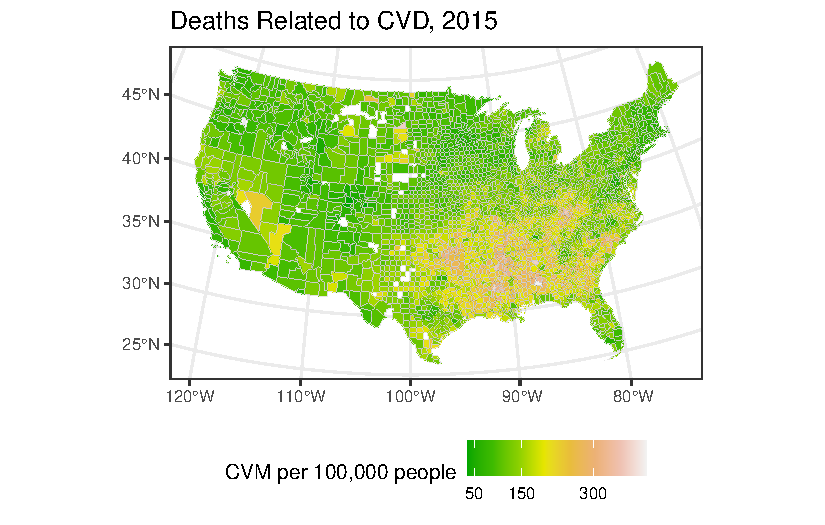
\includegraphics{report_files/figure-pdf/fig-1-1.pdf}

}

\caption{\label{fig-1}Higher death rates can be seen in Stroke Belt
region for 2015}

\end{figure}%

\section{Results}\label{results}

\subsection{Regression Summary}\label{regression-summary}

The GWR regression showed two models: global regression and GWR
regression output. They show the relationships between socioeconomic,
demographic, and environmental variables and death rates. The first is a
global regression model that does not consider spatial correlation
despite revealing that all predictors are statistically significant.
Hence, while the model does suggest that our variables are indeed
important, the global model may overlook local variations that are
crucial in understanding the true nature of the data. This can be seen
in Figure~\ref{fig-2}, which shows the residual of the global model, and
there appears to be a spatial pattern to the residuals, with specific
areas showing clusters of higher residuals and the other regions showing
clusters of lower residuals. This clustering of residuals suggests that
the global regression model may not be capturing all the spatial
variation in the data. This implies that the relationship between the
independent and dependent variables might differ across different
locations.

On the other hand, the geographically weighted regression (GWR) model
incorporates spatial variation, which is a critical factor given the
data context. We can see that the AIC and BIC values are lower for the
GWR regression than the Global regression, which makes it the most
preferred model given the data.~ In summary, by accommodating the
spatial component present in the data, the GWR model provides a more
realistic interpretation of how various factors influence death rates
across different regions.

\begin{figure}

\centering{

\captionsetup{labelsep=none}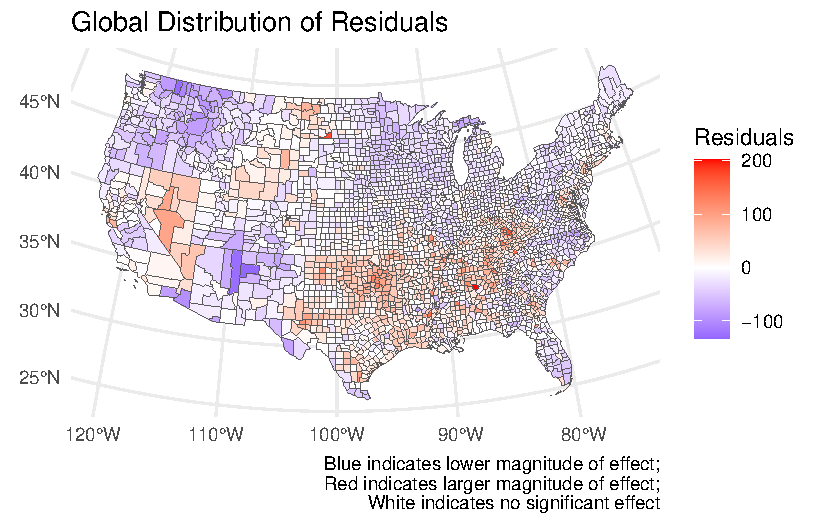
\includegraphics{report_files/figure-pdf/fig-2-1.pdf}

}

\caption{\label{fig-2}}

\end{figure}%

\subsection{Local Significance Plots}\label{local-significance-plots}

In Figure~\ref{fig-1}, the plot shows an exploratory data analysis (EDA)
plot, specifically a choropleth map displaying the number of deaths from
cardiovascular disease (CVD) per 100,000 people across the contiguous
United States for the year 2015. The particulate concentrations include
all the covariates mentioned in the methods section. The regions along
the higher latitudes (nearing 45 N) and towards the eastern section
(approaching 80 W) display darker shades, suggesting higher CVD death
rates in these areas, specifically the midwest and southwest regions.~

Figure~\ref{fig-3} represents the local significance and magnitude of
the `\% White' demographic parameter on cardiovascular disease outcomes.
We plotted for the local significance and magnitude because it can help
identify areas where the predictor variable has a stronger or weaker
influence on the outcome, leading to targeted insights that would not be
possible with a global model. From the plot, the prominent dark purple
areas in the central part of the country, extending towards the
southeastern regions, indicate a significant negative correlation
between the percentage of the white population and CVD outcomes in these
areas. Like the Northwest region, however, there are few areas,
particularly in the southwest near New Mexico and Arizona, where there
are positively correlated to CVD death rate, with the white regions of
counties suggesting no significance and this is white region is similar
for all the figures.

Figure~\ref{fig-4} represents the local significance and magnitude of
the `\% African' demographic parameter on cardiovascular disease
outcomes. From the plot, areas located approximately in the northern
central region indicate a significant positive correlation to CVD rate,
and areas, notably in the central to southeastern areas of the map,
suggest a significant negative correlation.

Figure~\ref{fig-5} represents the local significance and magnitude of
the `\% Hispanic' demographic parameter on cardiovascular disease
outcomes. From the plot, areas across the central and southeastern
regions are shaded in purple, suggesting a significant negative
correlation between the percentage of the Hispanic population and CVD
outcomes. The isolated red patches in the north-central region indicate
areas where an increased Hispanic population correlates with higher CVD
outcomes.~

Figure~\ref{fig-6} represents the local significance and magnitude of
the `\% Asian' demographic parameter on cardiovascular disease outcomes.
From the plot, a substantial portion of the map, particularly across the
central to eastern regions, is colored in various shades of purple. This
suggests that in these areas, an increased percentage of the Asian
population correlates with lower CVD outcomes. However, there are some
parts of the West where higher percentages of the Asian population are
associated with an increase in CVD outcomes.~

Figure~\ref{fig-7} represents the local significance and magnitude of
the ``\%p2.5 air quality'' parameter on cardiovascular disease outcomes.
From the plot, in the southern and northeastern regions, there increased
levels of PM2.5 colored as red in the plot, meaning they are associated
with higher rates of CVD. There are some regions in the West where it
was negatively correlated with CVD.

Figure~\ref{fig-8} represents the local significance and magnitude of
the ``median income'' parameter on cardiovascular disease outcomes. From
the plot, most of the region suggests a significant negative correlation
between the median income parameter and CVD outcomes. However, some
parts of Texas indicate a positive correlation to CVD outcomes.~

Figure~\ref{fig-9} represents the local significance and magnitude of
the ``Unemployment'' parameter on cardiovascular disease outcomes. From
the plot, there is a positive correlation to CVD rates in most of the
central region, and in the southwest region, there is a negative
correlation.

\begin{figure}

\begin{minipage}{0.50\linewidth}

\centering{

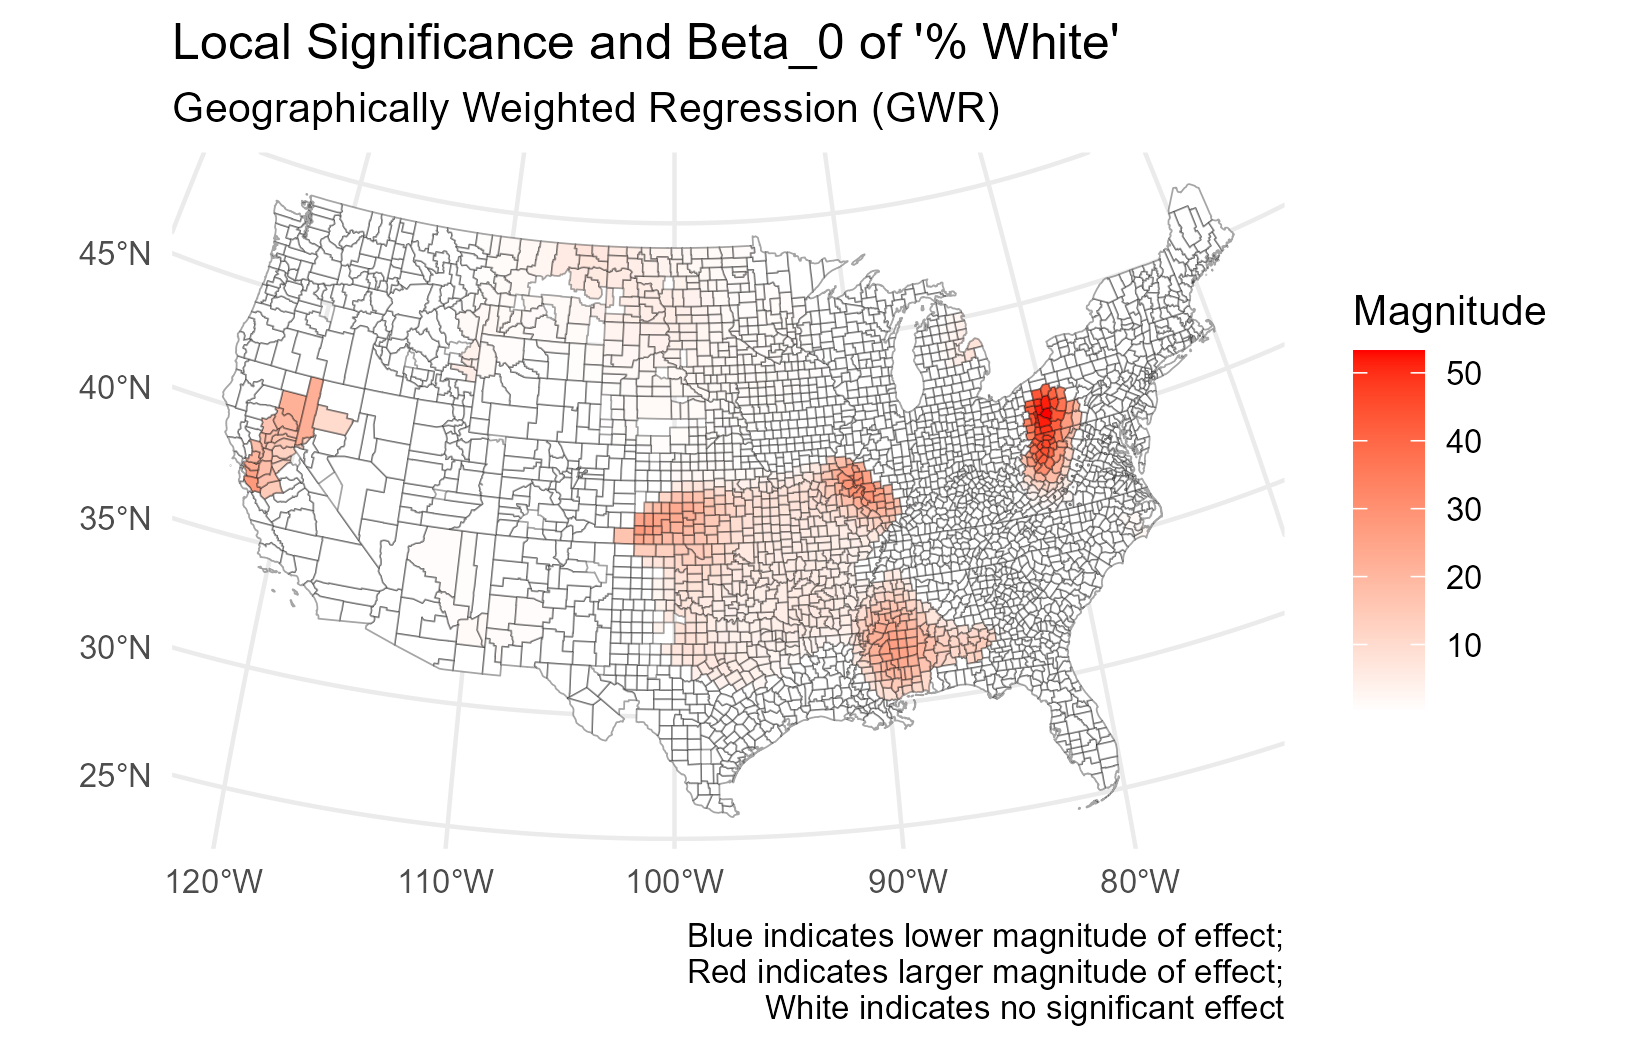
\includegraphics{PresentationPhotos/whiteplot.png}

}

\subcaption{\label{fig-3}Figure 3a: Strong effect in southern New
England area}

\end{minipage}%
%
\begin{minipage}{0.50\linewidth}

\centering{

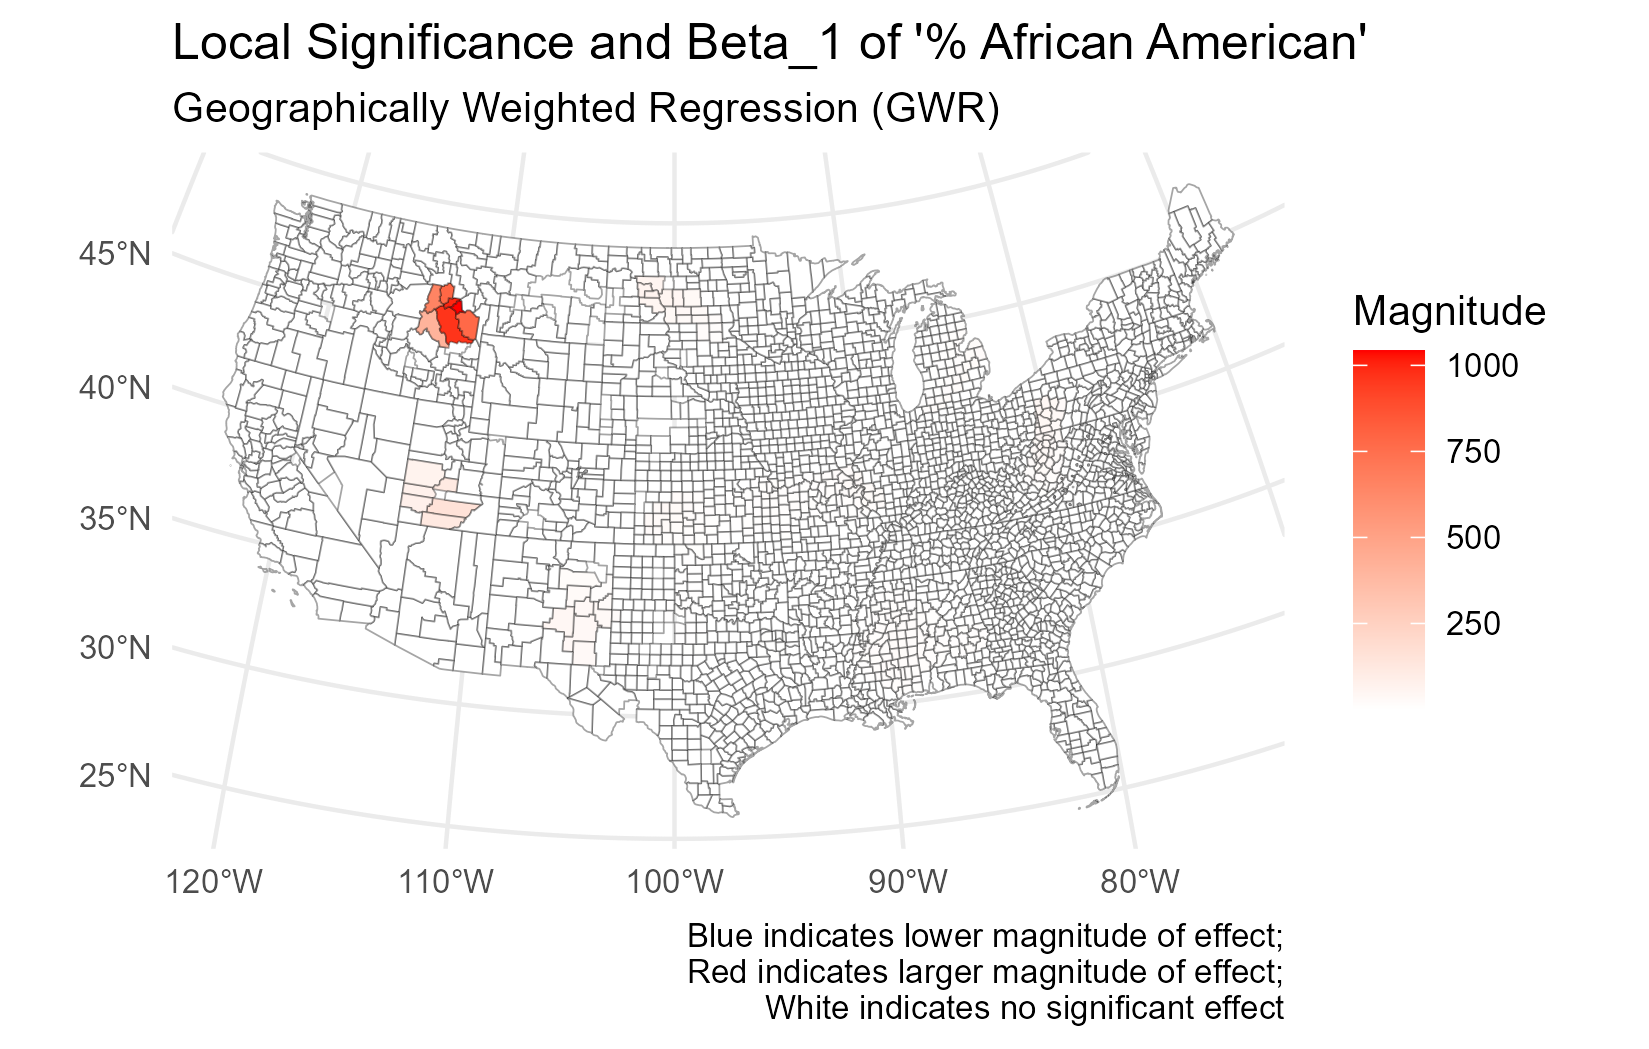
\includegraphics{PresentationPhotos/blackplot.png}

}

\subcaption{\label{fig-4}Figure 3b: Significant positive effect in Idaho
region}

\end{minipage}%
\newline
\begin{minipage}{0.50\linewidth}

\centering{

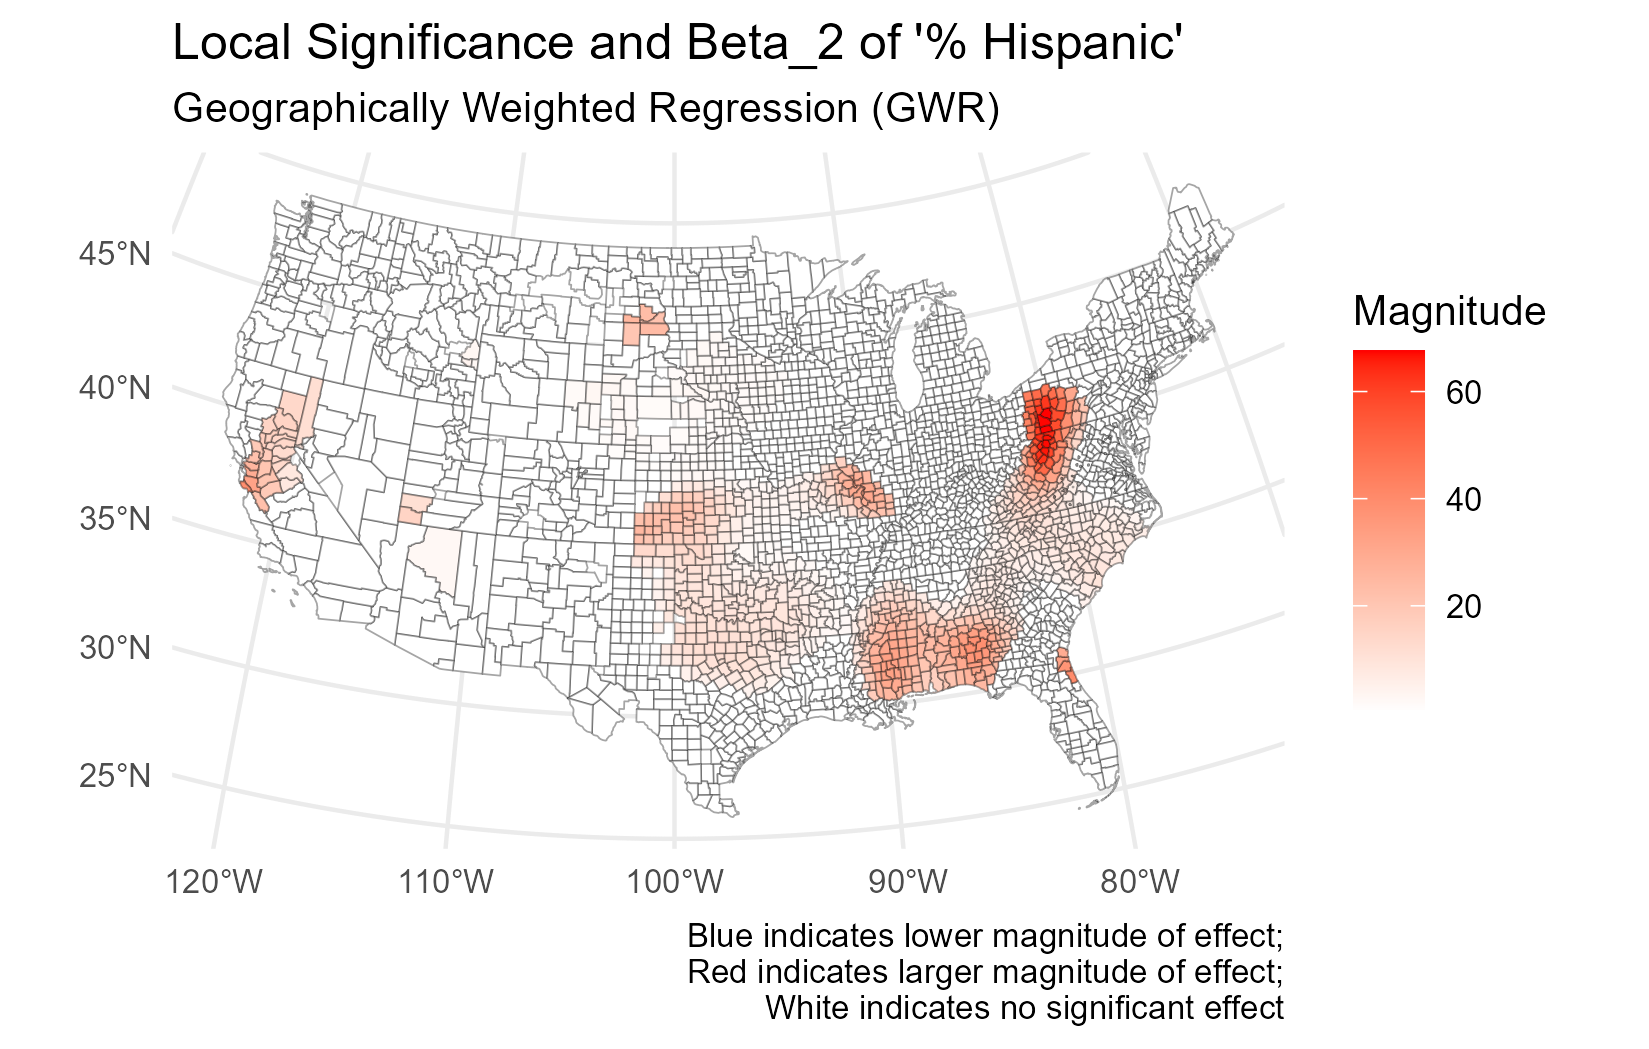
\includegraphics{PresentationPhotos/hispanplot.png}

}

\subcaption{\label{fig-5}Figure 3c: Positive effect focused in New
England}

\end{minipage}%
%
\begin{minipage}{0.50\linewidth}

\centering{

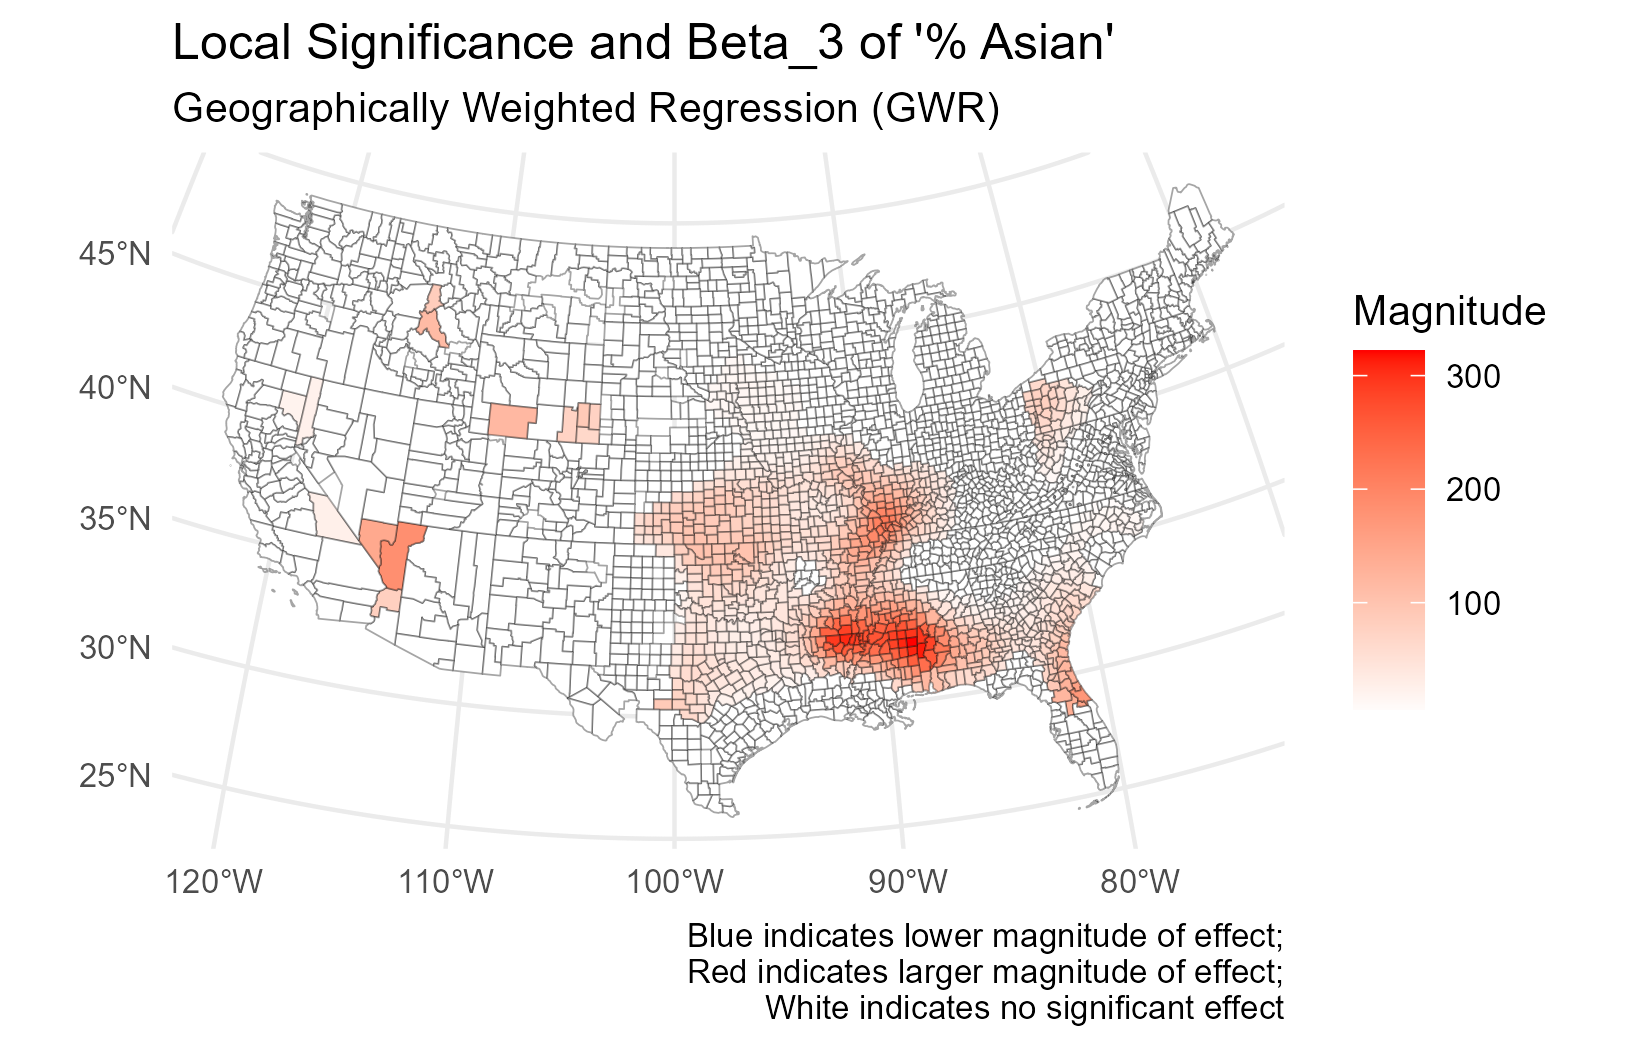
\includegraphics{PresentationPhotos/asianplot.png}

}

\subcaption{\label{fig-6}Figure 3d: Strong positive effects focused in
western Stroke Belt, minor positive effects through region}

\end{minipage}%

\end{figure}%

\begin{figure}

\centering{

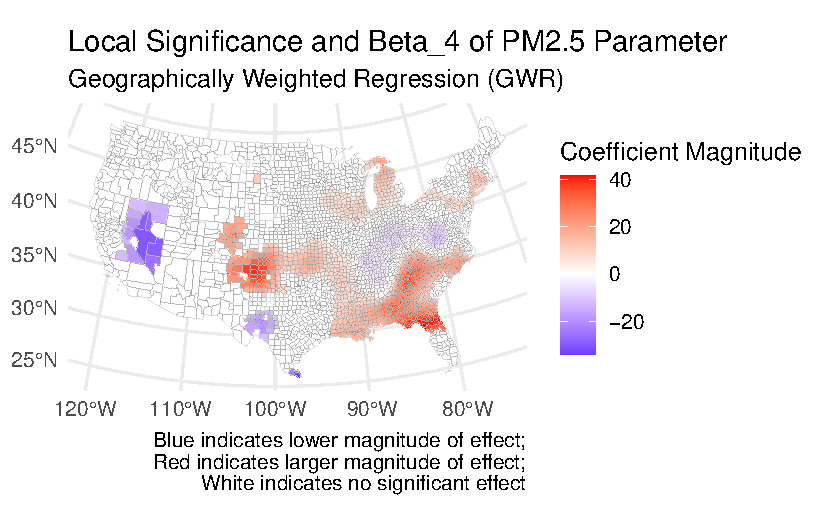
\includegraphics{report_files/figure-pdf/fig-7-1.pdf}

}

\caption{\label{fig-7}Higher effect in south and northeast. Negative
effect in the west.}

\end{figure}%

\begin{figure}

\begin{minipage}{0.50\linewidth}

\centering{

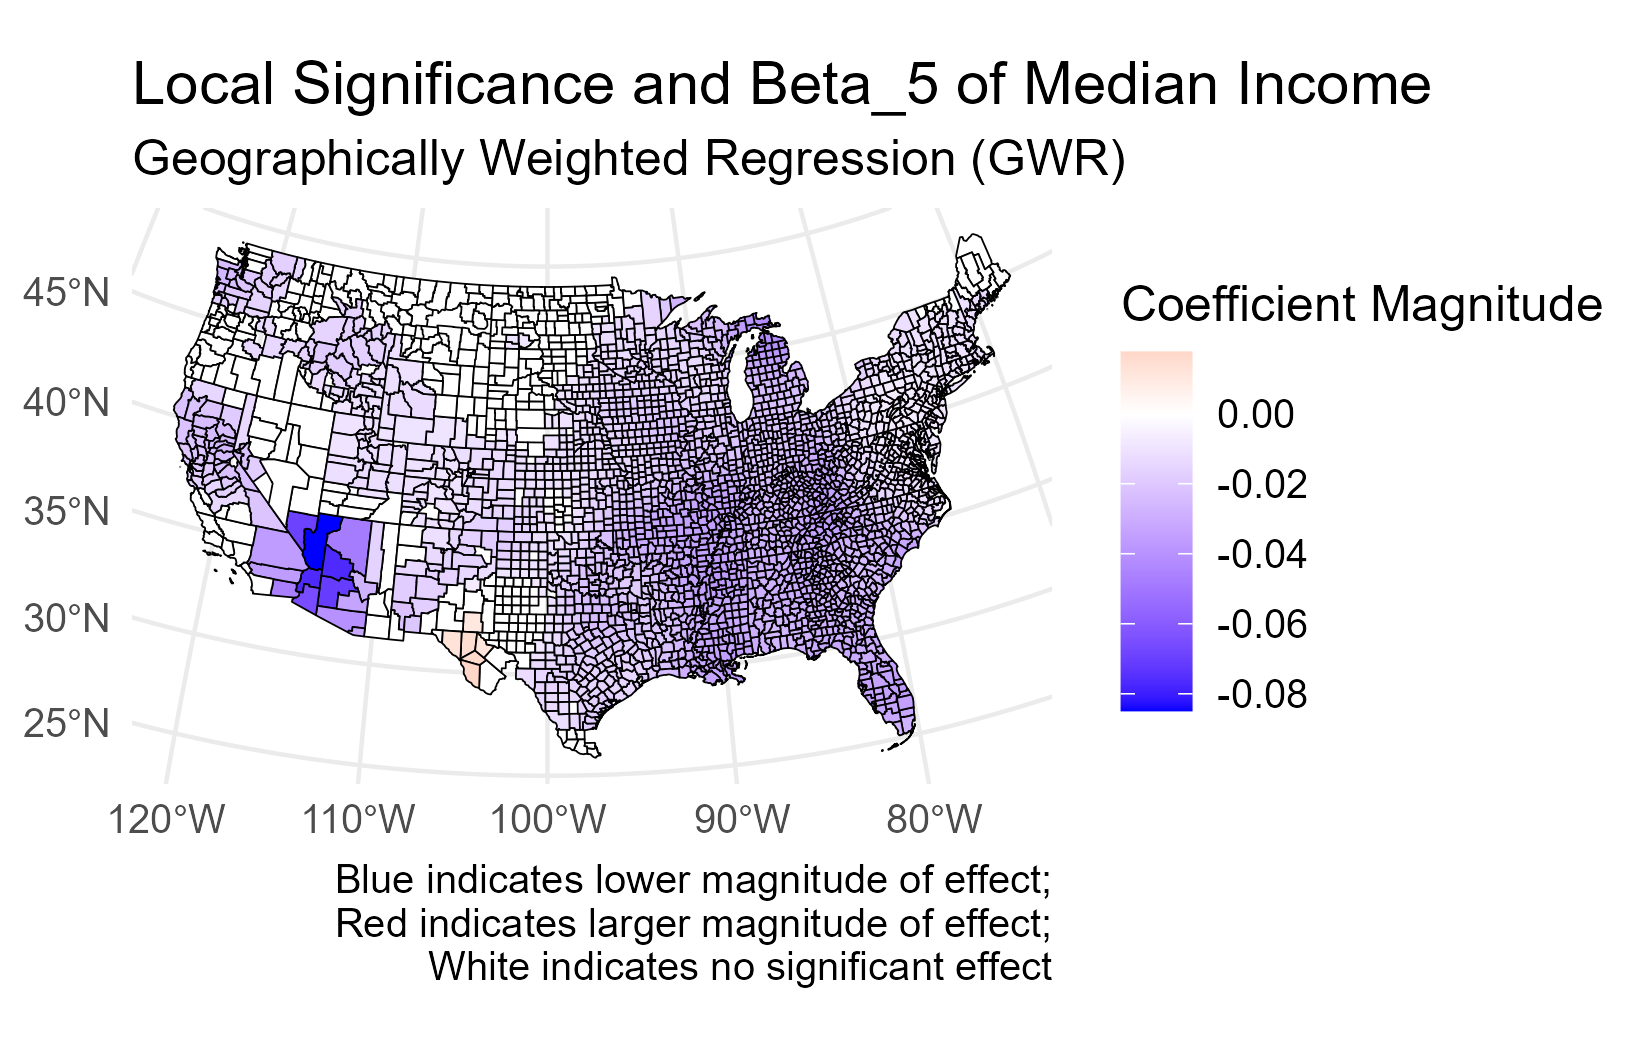
\includegraphics{PresentationPhotos/medIncomePlot.png}

}

\subcaption{\label{fig-8}Figure 5a: As expected, median income has a
consistent negative relationship with CVM}

\end{minipage}%
%
\begin{minipage}{0.50\linewidth}

\centering{

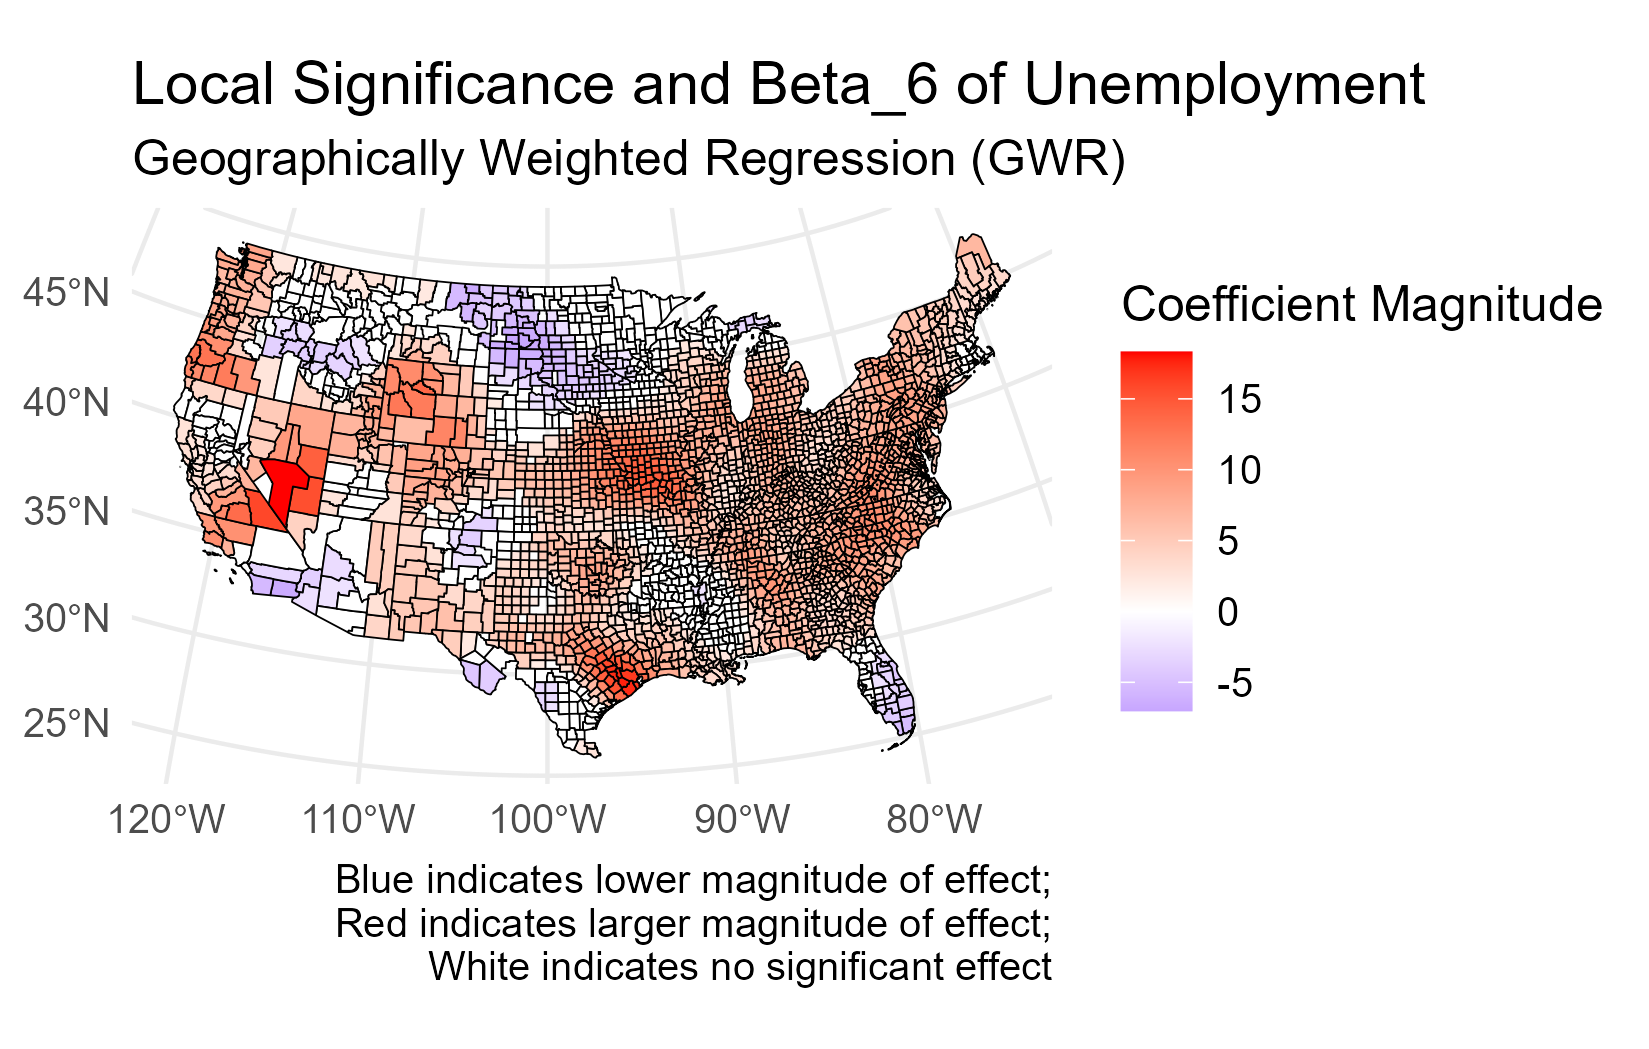
\includegraphics{PresentationPhotos/unemployPlot.png}

}

\subcaption{\label{fig-9}Figure 5b: Consistently positive relationship
in central regions, however negative patches exist in Florida and
northern states}

\end{minipage}%

\end{figure}%

\section{Discussion}\label{discussion}

The purpose of this study was to fill a gap in prior studies where the
impacts of CVD were primarily studied within the Stroke Belt, rather
than the country at large.

Our goal was to put our findings towards answering the following
question: what are the socioeconomic and environmental factors affecting
CVD rates in the United States?

These maps reveal that the relationships between race, socio-economic
factors, environmental quality, and death rates are complex and highly
localized. The significance and strength of these relationships vary
considerably across different parts of the United States. In contrast,
some of the socio-economic factors such as median income show
widespread, consistent significance, implying that the significance of
the relationship with CVD outcomes is nearly constant across various
locations. This differs from the heterogeneous local significance that
we observed in the majority of our other variables.

Another factor to consider from the plots is the percentage of each race
that inhabits each county. We can observe that for African Americans,
Hispanics, and Asians that the impacts are significant in localized
areas of the country, which may reflect underlying health disparities in
access to medical care. One limitation of race percentages is the
misreporting of medical records affecting minorities (Tabb et al. 2020).
However, this oversight lends further credence to the fact that
intervention is needed in order to combat racial health disparities. We
can look at the Variance Inflation Factor (VIF) to determine if
multi-collinearity has an impact on our results:

\begin{table}

\caption{\label{tbl-10}}

\centering{

\captionsetup{labelsep=none}

\begin{tabular}{rrrrrrr}
  \hline
\%White & \%Black & \%Hispanic & \%Asian & PM2.5 & MedIncome & Unemployment \\ 
  \hline
183.00 & 196.00 & 7.00 & 3.00 & 1.00 & 2.00 & 3.00 \\ 
  81.00 & 94.00 & 4.00 & 3.00 & 2.00 & 3.00 & 3.00 \\ 
  302.00 & 314.00 & 17.00 & 4.00 & 1.00 & 2.00 & 2.00 \\ 
  141.00 & 151.00 & 5.00 & 2.00 & 1.00 & 2.00 & 3.00 \\ 
  132.00 & 128.00 & 8.00 & 3.00 & 1.00 & 2.00 & 2.00 \\ 
  283.00 & 294.00 & 14.00 & 4.00 & 1.00 & 2.00 & 2.00 \\ 
   \hline
\end{tabular}

}

\end{table}%

Typically, when examining the VIF of a GWR model, we want the
coefficients for each of the seven columns--which represent our seven
independent variables--to be less than 15. We can see in
Table~\ref{tbl-10} that this standard holds for most cases of the
columns outside the \% White column, which has extremely high values.
This represents a limitation in our model, as it shows multicollinearity
with respect to the white and black variables, however, this is to be
expected given that the racial variables we are using sum up to one. An
adjustment to the model could be made in a future study to eliminate the
\% White variable and aggregate the other three into a single \%
Non-White variable. .

The concentration of PM2.5 and the consequential reduction in air
quality has a significant impact localized in the central and
southeastern regions of the United States, suggesting environmental
health concerns that might require region-specific intervention.~

We have shown that by using a GWR model to analyze the relationship
between CVM and socioeconomic covariates, the factors that have the most
significant impact on death rates vary by area of the country. This
highlights the need to identify methods of intervention in order to curb
one of the deadliest groups of diseases on the planet (Marlow 1994).

\section{Appendix}\label{appendix}

The R code used for this study can be found in our public GitHub
repository: \url{https://github.com/jbooc117/STAT489-Project.git}.

\subsection{Simulation Study Figures}\label{simulation-study-figures}

\begin{longtable}[]{@{}lll@{}}
\toprule\noalign{}
Moran I Statistic & Expectation & Variance \\
\midrule\noalign{}
\endhead
\bottomrule\noalign{}
\endlastfoot
0.3010445156 & 0.0003274394 & 0.0001178233 \\
\end{longtable}

\begin{figure}

\centering{

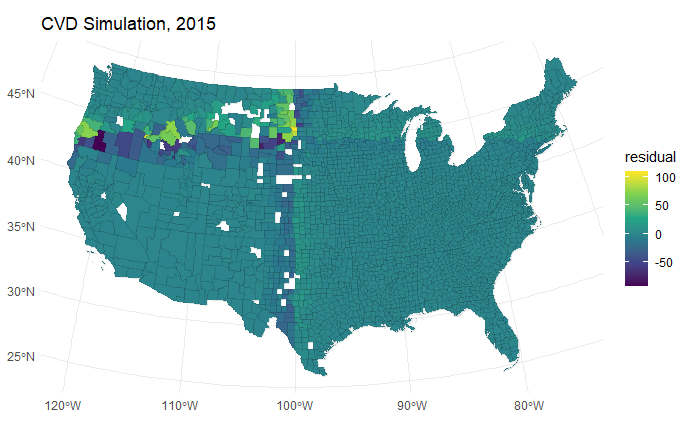
\includegraphics{PresentationPhotos/simplot.png}

}

\caption{\label{fig-A1}Division of country into four quadrants shows the
effectiveness of the GWR model}

\end{figure}%

\newpage{}

\section*{References}\label{references}
\addcontentsline{toc}{section}{References}

\phantomsection\label{refs}
\begin{CSLReferences}{1}{0}
\bibitem[\citeproctext]{ref-gebreabExploringRacialDisparities2012}
Gebreab, Samson Y., and Ana V. Diez Roux. 2012. {``Exploring Racial
Disparities in {CHD} Mortality Between Blacks and Whites Across the
{United} {States}: {A} Geographically Weighted Regression Approach.''}
\emph{Health \& Place} 18 (5): 1006--14.
\url{https://doi.org/10.1016/j.healthplace.2012.06.006}.

\bibitem[\citeproctext]{ref-liuAnalysisShortTermEffects2020}
Liu, Yi, Jingjie Sun, Yannong Gou, Xiubin Sun, Dandan Zhang, and Fuzhong
Xue. 2020. {``Analysis of {Short}-{Term} {Effects} of {Air} {Pollution}
on {Cardiovascular} {Disease} {Using} {Bayesian} {Spatio}-{Temporal}
{Models}.''} \emph{International Journal of Environmental Research and
Public Health} 17 (3): 879.
\url{https://doi.org/10.3390/ijerph17030879}.

\bibitem[\citeproctext]{ref-Marlow1994}
Marlow, Hilary F. 1994. {``The Pharmaceutical Industry Viewpoint.''}
\emph{Cardiology} 85 (1): 102--12.
\url{https://doi.org/10.1159/000176769}.

\bibitem[\citeproctext]{ref-singhSpatiotemporalDemographicTrends2019}
Singh, Gitanjali M., Ninon Becquart, Melissa Cruz, Andrea Acevedo,
Dariush Mozaffarian, and Elena N. Naumova. 2019. {``Spatiotemporal and
{Demographic} {Trends} and {Disparities} in {Cardiovascular} {Disease}
{Among} {Older} {Adults} in the {United} {States} {Based} on 181
{Million} {Hospitalization} {Records}.''} \emph{Journal of the American
Heart Association} 8 (21): e012727.
\url{https://doi.org/10.1161/JAHA.119.012727}.

\bibitem[\citeproctext]{ref-tabbExploringSpatialPatterning2020}
Tabb, Loni Philip, Angel Ortiz, Suzanne Judd, Mary Cushman, and Leslie
A. McClure. 2020. {``Exploring the {Spatial} {Patterning} in {Racial}
{Differences} in {Cardiovascular} {Health} {Between} {Blacks} and
{Whites} {Across} the {United} {States}: {The} {REGARDS} {Study}.''}
\emph{Journal of the American Heart Association} 9 (9): e016556.
\url{https://doi.org/10.1161/JAHA.120.016556}.

\bibitem[\citeproctext]{ref-terryTrendsCardiovascularDisease2023}
Terry, Katrina, Mohamed Makhlouf, Salah E. Altarabsheh, Vaishali Deo,
Fanny Petermann-Rocha, Yakov Elgudin, Khurram Nasir, Sanjay Rajagopalan,
Sadeer Al-Kindi, and Salil Deo. 2023. {``Trends in {Cardiovascular}
{Disease} {Mortality} by {County}-{Level} {Social} {Vulnerability}
{Index} in the {United} {States}.''} \emph{Journal of the American Heart
Association} 12 (20): e030290.
\url{https://doi.org/10.1161/JAHA.123.030290}.

\bibitem[\citeproctext]{ref-warsitoRobustGeographicallyWeighted2018}
Warsito, Budi, Hasbi Yasin, Dwi Ispriyanti, and Abdul Hoyyi. 2018.
{``Robust Geographically Weighted Regression of Modeling the {Air}
{Polluter} {Standard} {Index} ({APSI}).''} \emph{Journal of Physics:
Conference Series} 1025 (May): 012096.
\url{https://doi.org/10.1088/1742-6596/1025/1/012096}.

\bibitem[\citeproctext]{ref-zelkoGeographicallyWeightedModeling2023}
Zelko, Andrea, Pedro R. V. O. Salerno, Sadeer Al-Kindi, Fredrick Ho,
Fanny Petermann Rocha, Khurram Nasir, Sanjay Rajagopalan, Salil Deo, and
Naveed Sattar. 2023. {``Geographically {Weighted} {Modeling} to
{Explore} {Social} and {Environmental} {Factors} {Affecting}
{County}-{Level} {Cardiovascular} {Mortality} in {People} {With}
{Diabetes} in the {United} {States}: {A} {Cross}-{Sectional}
{Analysis}.''} \emph{The American Journal of Cardiology} 209 (December):
193--98. \url{https://doi.org/10.1016/j.amjcard.2023.09.084}.

\end{CSLReferences}



\end{document}
